

\chapter{Introduction}
"Physical Fitness is the first requisite of happiness" - Joseph Pilates
Heart disease is one of the leading causes of death in the world. Heart disease is caused by obesity and poor lifestyle choices. Sometimes heart diseases can be hereditary as well. Needless to say, it is important to maintain good heart health. The aim of this project is to develop a reliable machine learning model to determine whether a patient will need to visit a physician and whether a patient is developing an underlying heart condition. 
\\
Health care are of two types :-
\\1. Reactive Health care, and
\\2. Preventive Health care
\\While Reactive health care is given when symptoms of a disease is observed, Preventive health care stops conditions from occurring. Doctors agree that preventive health care is cheaper and better than reactive health care. It is easier to keep people healthy rather than curing a disease.
\\ 
In India, often times a patient may not be able to access proper preventative health care. This may be due to lack of  time or money. Furthermore, experienced doctors in India are scarce and have a long queues of patients. A patient might not want preventive health care in such situations as it is difficult and time consuming to schedule an appointment with the doctor.  
\\
The project discussed in this report tries to address this issue. The system encourages people to take the path of preventive health care rather than reactive health care by making the former more accessible with respect to time and money. Heart Diseases can be monitored in their initial stages and can help prevent further complications. Lastly, this project has been developed for people to maintain a healthy lifestyle.
\\
This project tries to predict whether a patient needs to visit a physician. Several machine learning algorithms have been used to access which algorithm provides the most accurate results. It must be noted that in commercial use, it is safer to have a bias of trying to send a patient to the physician.


\section{Motivation}
Good health is a human right. Poor people cannot always afford preventive health care. The best way to make health care available to all is by making it cheap and fast. The project was developed with the intention to make health care cheaper, accurate and more accessible.

\section{Sensors}
\begin{enumerate}
\item ESP8266 12E wi-fi/Node MCU	
\item 4/8/16 channel Relay Board				
\item USB TTL Serial Adapter
\item PIR Motion sensors 
\end{enumerate}

\subsection{Thermostats and HVAC controls}
Common thermostats and HVAC controls  are:
\begin{itemize}
\item 	Humidity sensing and control  
\item 	Temperature sensors and controllers    
\item 	Weather stations and sensors  
\end{itemize}

\subsection{Example Figure}
An example figure insertion is presented  in  Figure \ref{fig1}.

\begin{figure}[H]
\begin{center}
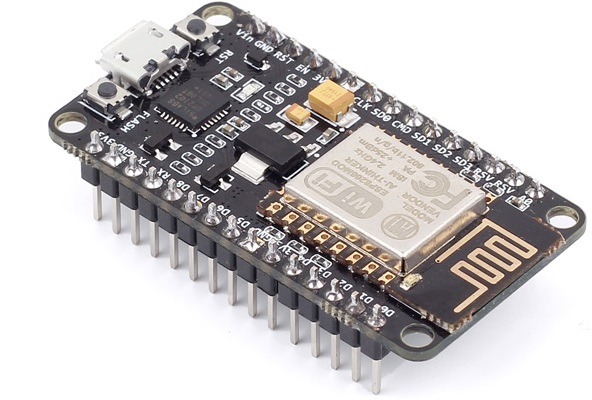
\includegraphics[width=0.8\textwidth]{fig1}
\end{center}
\caption{NodeMCU Microcontroller}
\label{fig1}
\end{figure}

\subsection{Example Referencing}
An example of inserting references in latex \cite{7890229} \cite{swapnil2016}. 

\section{Chapter Summary}
In this chapter, .....  
